\documentclass[a4paper,12pt]{article} 
\usepackage[T2A]{fontenc}			
\usepackage[utf8]{inputenc}			
\usepackage[english,russian]{babel}	
\usepackage{amsmath,amsfonts,amssymb,amsthm,mathtools} 
\usepackage[colorlinks, linkcolor = blue]{hyperref}
\usepackage{upgreek}
\usepackage[left=2cm,right=2cm,top=2cm,bottom=3cm,bindingoffset=0cm]{geometry}
\usepackage{multirow}
\usepackage{graphicx}
\usepackage{xcolor}
\usepackage{multirow}
\usepackage{pgfplots}
\usepackage{pgfplotstable}
\pgfplotsset{compat=1.9}

\pgfplotstableset{ %
        create on use/SquareLight/.style={
                create col/expr={\thisrow{Dark}}}
}

\author{Шелихов Дмитрий\\Группа Б01-305}

\title{\textbf{Работа 3.7.1\\Скин-эффект в полом цилиндре}} 
\date{\today}

\begin{document} 

\maketitle

\textbf{Цель работы:} исследовать явление проникновения переменного магнитного поля в медный полый цилиндр. \\
\par\textbf{В работе используются:} генератор сигналов АКИП-3420, соленоид, намотанный на полый цилиндрический каркас, медный экран в виде полого цилиндра, измерительная катушка, амперметр, вольтметр, двухканальный осциллограф GOS-620, RLC-метр. \\

\par\textbf{Теоретические сведения}\\

Считаем цилиндр достаточно длинным, так что в нем можно пренебречь краевыми эффектами. Тогда магнитное поле $\vec{H}$ всюду направлено по оси системы Oz, а вихревое электрическое поле $\vec{E}$ будет всюду перпендикулярно радиусу. (линии поля образуют соосные окружности)

\begin{figure}
\center{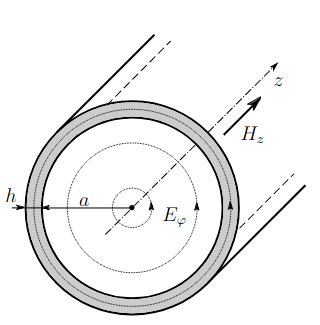
\includegraphics[width=.6\textwidth]{1.png}}[H]
\caption{Электрическое и магнитное поле в тонкостенном цилиндре}
\end{figure}

Все величины считаем колеблющимися по гармоническому закону с некоторой частотой $\omega$, задаваемой частотой колебания тока в соленоиде. Тогда: 

$$H_z = H(r)e^{i\omega t}, E_z = E(r)e^{i\omega t}$$

На границе цилиндра должны быть непрерывны касательные к поверхности компоненты как $\vec{E}$, так и $\vec{H}$ => E(r) и H(r) непрерывны во всей исследуемой области. \\
Пусть длинный полый цилиндр имеет радиус a и толщину стенки h << a. Последнее условие позволяет для описания поля внутри стенки ограничиться одномерным приближением. При этом для полного решения задачи необходимо вычислить и распределение поля внутри цилиндра. \\
Внутри цилиндра ток отсутсвует => магнитное поле там является однородным $H_z(r,t) = H_1e^{i\omega t}$, где $H_1$ = const - амплитуда поля на внутренней поверхности цилиндра. Для нахождения вихревого электрического поля воспользуемся законом электромагнитной индукции в интегральной форме: 
$$E_{\varphi} \cdot 2\pi r = - {\mu}_0\pi r^2 \cdot \frac{dH_z}{dt} \rightarrow E(r) = -\frac{1}{2}{\mu}_0 r \cdot i\omega H_1$$. 

Откуда получаем связь амплитуд колебаний электрического и магнитного полей на внутренней (r = a) границе цилиндра: 

$$ E_1 = -\frac{1}{2}i\omega a{\mu}_0 H_1 $$

\begin{figure}[htp]
\center{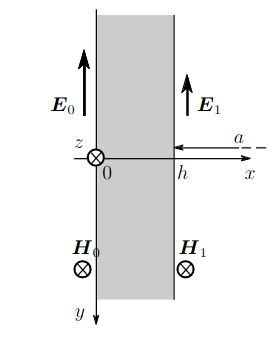
\includegraphics[width=.4\textwidth]{2.png}}
\caption{Поле в стенке цилиндра}
\end{figure}

Поле внутри тонкой стенки цилиндра описывается уравнением скин-эффекта в плоском случае:
$$\frac{d^2 H}{dx^2} = i\omega \sigma {\mu}_0 H$$

Где для медного цилиндра $\mu \approx$ 1. 

Граничные условия: 

$$H(0) = H_1, H(h) = H_1$$. 

Решением дифференциального уравнения скин-эффекта с учетом граничных условий при x = h является: 

$$H_1 = \frac{H_0}{ch(\alpha h) + \frac{1}{2}\alpha a sh(\alpha h)}$$

где $\alpha = \frac{\sqrt{2}}{\delta}e^{i\pi/4}$, $\delta = \sqrt{\frac{2}{\omega \sigma {\mu}_0}}$ - глубина скин-слоя. 

Предельные случаи: \\ 

1) При малых частотах $\delta >> h$, тогда $|\alpha h|$ << 1, поэтому $ch\alpha h \approx 1$, $sh \alpha h \approx \alpha h$ и 

$$H_1 \approx \frac{H_0}{1+i\frac{ah}{{\delta}^2}}$$

Отношение модулей амплитуд: 

$$\frac{|H_1|}{|H_0|} = \frac{1}{\sqrt{1 + \frac{1}{4}(ah\sigma{\mu}_0\omega})^2}$$

При этом колебания $H_1$ отстают по фазе от $H_0$ на угол $\psi$:

$$tg(\psi) = \frac{ah}{{\delta}^2}$$

2) При достаточно больших частотах $\delta$ << h. Тогда sh($\alpha h$) $\approx$ ch($\alpha h$) $\approx$ $\frac{1}{2}e^{\alpha h}$.

Отношение амплитуд: 

$$\frac{H_1}{H_0} = \frac{4e^{-\alpha h}}{\alpha a} = \frac{2\sqrt \delta}{a} \cdot e^{-\frac{h}{\delta}}e^{-i(\frac{\pi}{4} + \frac{h}{\delta})}$$. 

Запаздывание поля внутри, чем поля снаружи на: 

$$\psi = \frac{\pi}{4} + h\sqrt{\frac{\omega \sigma {\mu}_0}{2}}$$

\begin{figure}[htp]
\center{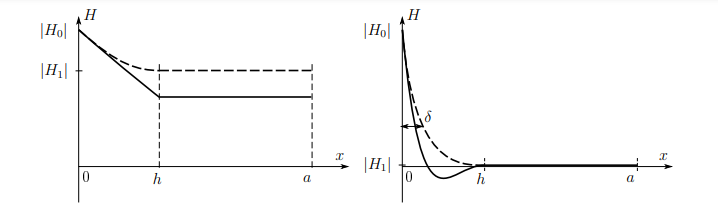
\includegraphics[width=.6\textwidth]{4.png}}
\caption{Распределение амплитуды колебаний магнитного поля и его мгновенного значения при некотором t в зависимости от расстояния x до внешней стенки цилиндра. Слева - низкие частоты, справа - высокие частоты}
\end{figure}

\par\textbf{Экспериментальная установка}

Переменное магнитное поле создается с помощью соленодиа, намотанного на цилиндрический каркас, который подключается к генератору сигналов. Внутри каркаса расположен медный экран в виде полого цилиндра. \\ 
1) Цифровым амперметром измеряется действующее значение переменного тока в цепи соленоида. \\
2) Цифровым вольтметром измеряется действующее напряжение на измерительной катушке 4. \\
3) На канал Y осциллографа податся напряжение с измерительной катушки, а на X - напряжение резистора R, которое пропорционально току в соленоиде. С помощью осциллографа будем определять сдвиг фаз между напряжениями. 

\begin{figure}[htp]
\center{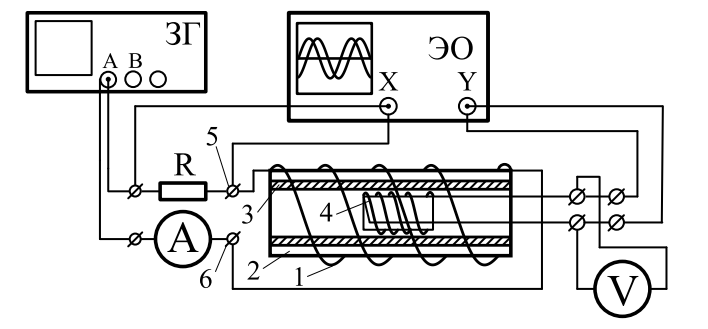
\includegraphics[width=.6\textwidth]{3.png}}
\caption{Экспериментальная установка для изучения скин-эффекта}
\end{figure}

Для определения проводимости $\sigma$ по изменению L катушки используем RLC-метр 

\begin{figure}[htp]
\center{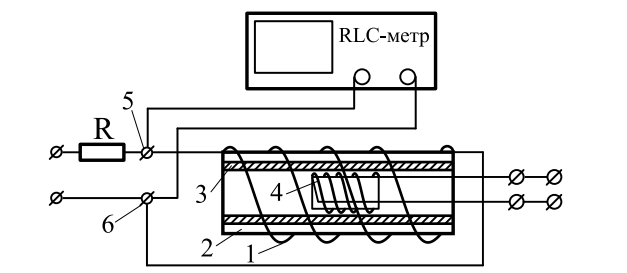
\includegraphics[width=.6\textwidth]{5.png}}
\caption{Схема подключения RLC-метра}
\end{figure}

\par\textbf{Измерение отношения амплитуд магнитного поля внутри и вне экрана}

С помощью вольтметра V измеряется действующее значение ЭДС индукции, которое возникает в измерительной катушке, находящейся в переменном магнитном поле. 

$$U = -SN\frac{dB_1(t)}{dt} = -i\omega {\mu}_0SNH_1e^{i\omega t}$$ - комплексная амплитуда ЭДС индукции в измерительной катушке. 

Вольтметр показывает действующее значение: 

$$ U = \frac{SN\omega}{\sqrt{2}}{\mu}_0|H_1|$$

Откуда:

$$ \frac{|H_1|}{|H_0|} = const\cdot\frac{U}{\nu I}  $$

Неизвестную константу измеряем при малых частотах $\nu \rightarrow 0$, когда $\frac{|H_1|}{|H_0|} \rightarrow 1$. 

\par\textbf{Определение проводимости материала экрана по фазовому сдвигу}

Для определения $\sigma$ экрана будем использовать частотную зависимость фазового сдвига между магнитными полями внутри и вне экрана при низких и высоких частотах.//

Зависимость tg($\psi$) от $\nu$ линейна, причем аппроксимирующая прямая должна проходить через начало координат. В области больших частот $\nu >> 1/(\pi h^2 \sigma {\mu}_0)$ зависимость $\psi(\sqrt{\nu}-\pi/4)$ аппроксимируется прямой, проходящей через начало координат. По наклону этих прямых можно вычислить проводимость материала экрана. \\

Заметим, что на входной канал Y осциллографа подается сигнал с измерительной катушки, который пропорционален производной поля внутри экрана по времени, поэтому появляется дополнительный сдвиг по фазе на $\pi/2$. Поэтому измеренный по осциллографу сдвиг по фазе между двумя синусоидами будет на $\pi/2$ больше фазового сдвига между магнитными полями вне и внутри экрана: 

$$\varphi = \psi + \frac{\pi}{2}$$

\par\textbf{Влияние скин-эффекта на индуктивность катушки}

Из-за скин эффекта индуктивность соленоида с медным цилиндрическим экраном внутри будет зависеть от частоты тока. \\
Рассмотрим магнитный поток через катушку как сумму двух магнитных потоков: \\
1) Пронизивыющий область между катушкой и цилиндрическим экраном ${\Phi}_{out}$
2) Пронизывающий область за экраном ${\Phi}_{in}$

$$\Phi = {\Phi}_{in} + {\Phi}_{out} = H_0 S_0 + H_1 S_1 = LI$$

Индуктивность минимальна в случае, если ${\Phi}_{in} = 0$ (поле есть только во внешней области). При этом $L_{min} = \frac{{\Phi}_{out}}{I}$\\
Максимальная индуктивность катушки достигается при максимальном потоке поля во внутренней области (когда $H_0 = H_1$):\\
${\Phi}_{max} = {\Phi}_{out} + {\Phi}_{in_max} = H_0(S_0 + S_1) = L_{max}I_m$, где поток через внешнюю область равен $H_0 S_0 = L_{max}I_m$\\
Откуда получаем: \\

$$\frac{L_{max}-L}{L-L_{min}} = {(\pi ah {\mu}_0 \sigma \nu)}^2$$

Данная зависимость может быть аппроксимирована прямой, по углу наклона которой можно найти проводимость материала $\sigma$.

\par\textbf{Ход работы}

\par1) Оценим частоту $\nu_h$, при которой толщина стенок экрана равна скиновой длине h = $\delta$. Для оценки примем проводимость меди $\sigma \approx 5\cdot {10}^7$ Сименс/м и $\mu \approx 1$. Воспользуемся формулой:\\

$$ \omega = 2\pi {\nu}_h = \frac{2}{{\delta}^2 \sigma {\mu}_0}$$

\begin{center}
\begin{tabular}{|c|c|c|c|c|}
	\hline
	$\delta$, мм & $\sigma$, Сименс/м & $\mu_0$, Гн/м & $\mu$ & $\nu_h$, кГц\\  
	\hline
	1.5 & 5$\cdot {10}^7$ & 4$\pi\cdot {10}^{-7}$ & 1 & 2.23 \\
	\hline
\end{tabular}
\end{center}

\par2) Соберем установку согласно рис.4 и настроим приборы. Установим начальную частоту сигнала генератора $\approx 0.01 \nu_h = 22.3$ Гц, а амплитуду выходного сигнала A $\approx$ 7-8 В.

\par3) В области низких частот (от $\approx 0,01 \nu_h$ до $0,05 \nu_h$) получим зависимость отношения $\xi = \frac{U}{\nu I} \text{от частоты} \nu$. Для этого измерим силу тока в цепи соленоида и напряжение на измерительной катушке для не менее 10 значений частоты $\nu$ в выбранном диапазоне.\\

\begin{center}
\begin{tabular}{|c|c|c|}
	\hline
	I, мА & U, В & $\nu$, Гц \\
	\hline
	454.4 $\pm$ 0.1 & 0.140 $\pm$ 0.001 & 22.3 \\
	\hline
	451.5 $\pm$ 0.1 & 0.194 $\pm$ 0.001 & 31.3 \\
	\hline
	447.3 $\pm$ 0.1 & 0.245 $\pm$ 0.001 & 40.3 \\
	\hline
	442.3 $\pm$ 0.1 & 0.292 $\pm$ 0.001 & 49.3 \\
	\hline
	436.2 $\pm$ 0.1 & 0.335 $\pm$ 0.001 & 58.3 \\
	\hline
	430.3 $\pm$ 0.1 & 0.375 $\pm$ 0.001 & 67.3 \\
	\hline
	424.2 $\pm$ 0.1 & 0.411 $\pm$ 0.001 & 76.3 \\
	\hline
	418.0 $\pm$ 0.1 & 0.444 $\pm$ 0.001 & 85.3 \\
	\hline
	412.0 $\pm$ 0.1 & 0.473 $\pm$ 0.001 & 94.3 \\
	\hline 
	406.1 $\pm$ 0.1 & 0.499 $\pm$ 0.001 & 103.3 \\
	\hline 
	400.0 $\pm$ 0.1 & 0.522 $\pm$ 0.001 & 112.3 \\
	\hline
\end{tabular}
\end{center}

Величина $\xi$ прямо пропорциональна коэффициенту ослабления магнитного поля внутри экрана относительно поля снаружи: \\

$$ \xi = \xi_0|H_1|/|H_0| $$. 

\par4) Исследуем зависимость величины $\xi$ и фазового сдвига $\psi$ от частоты $\nu$ при низких частотах в диапазоне от $0.05 \nu_h до 0.5 \nu_h$. Для этого получим статичную и удобную для измерения картинку на экране осциллографа и измерим разность фаз между напряжениями на резисторе и на катушке для не менее 15 знаечний частоты $\nu$ в выбранном диапазоне, а также силу тока в цепи соленоида и напряжение на измерительной катушке. Проведем 5-7 измерений в диапазоне частот  (0.05 $\nu_h$ - 0.1 $\ni_h$) и 8-10 измерений в диапазоне (0.1-0.5 $\nu_h$).

\begin{center}
\begin{tabular}{|c|c|c|c|}
	\hline
	$\nu$, Гц & U, В & I, мА & $\Delta\varphi$, рад \\
	\hline
	111.5 & 0.519 $\pm$ 0.001 & 399.3 $\pm$ 0.1 & 1.10 $\pm$ 0.05 \\
	\hline
	129.5 & 0.558 $\pm$ 0.001 & 388.9 $\pm$ 0.1 & 1.13 $\pm$ 0.05 \\
	\hline 
	147.5 & 0.590 $\pm$ 0.001 & 379.8 $\pm$ 0.1 & 1.11 $\pm$ 0.06 \\
	\hline
	165.5 & 0.614 $\pm$ 0.001 & 371.8 $\pm$ 0.1 & 1.11 $\pm$ 0.07 \\
	\hline
	183.5 & 0.634 $\pm$ 0.001 & 364.7 $\pm$ 0.1 & 1.12 $\pm$ 0.08 \\
	\hline
	201.5 & 0.650 $\pm$ 0.001 & 358.7 $\pm$ 0.1 & 1.20 $\pm$ 0.04 \\
	\hline
	219.5 & 0.662 $\pm$ 0.001 & 353.3 $\pm$ 0.1 & 1.23 $\pm$ 0.05 \\
	\hline
	309.5 & 0.696 $\pm$ 0.001 & 333.8 $\pm$ 0.1 & 1.37 $\pm$ 0.07 \\
	\hline
	399.5 & 0.706 $\pm$ 0.001 & 322.5 $\pm$ 0.1 & 1.38 $\pm$ 0.09 \\
	\hline
	489.5 & 0.706 $\pm$ 0.001 & 314.1 $\pm$ 0.1 & 1.35 $\pm$ 0.11 \\
	\hline
	579.5 & 0.700 $\pm$ 0.001 & 306.8 $\pm$ 0.1 & 1.46 $\pm$ 0.05 \\
	\hline
	669.5 & 0.691 $\pm$ 0.001 & 300.0 $\pm$ 0.1 & 1.49 $\pm$ 0.06 \\
	\hline
	759.5 & 0.680 $\pm$ 0.001 & 293.3 $\pm$ 0.1 & 1.52 $\pm$ 0.07 \\
	\hline
	849.5 & 0.668 $\pm$ 0.001 & 286.6 $\pm$ 0.1 & 1.47 $\pm$ 0.08 \\
	\hline
	939.5 & 0.654 $\pm$ 0.001 & 279.9 $\pm$ 0.1 & 1.51 $\pm$ 0.09 \\
	\hline
	1029.5 & 0.640 $\pm$ 0.001 & 273.2 $\pm$ 0.1 & 1.54 $\pm$ 0.05 \\
	\hline
	1119.5 & 0.625 $\pm$ 0.001 & 266.4 $\pm$ 0.1 & 1.54 $\pm$ 0.05 \\
	\hline
\end{tabular}
\end{center}

\par5) Повторим измерения пункта 4 при высоких частотах в диапазоне (0.5$\nu_h$ - 15 $\nu_h$) 15-20 точек\\

\begin{center}
\begin{tabular}{|c|c|c|c|}
	\hline
	$\nu$, Гц & U, В & I, мА & $\frac{\Delta\varphi}{2}$, рад \\
	\hline
	1119.5 & 0.625 $\pm$ 0.001 & 266.4 $\pm$ 0.1 & 1.54 $\pm$ 0.05 \\
	\hline
	3219.5 & 0.342 $\pm$ 0.001 & 148.0 $\pm$ 0.1 & 1.67 $\pm$ 0.08 \\
	\hline
	5319.5 & 0.212 $\pm$ 0.001 & 95.9 $\pm$ 0.1 & 1.84 $\pm$ 0.05 \\
	\hline
	7419.5 & 0.146 $\pm$ 0.001 & 69.6 $\pm$ 0.1 & 1.94 $\pm$ 0.07\\
	\hline
	9519.5 & 0.103 $\pm$ 0.001 & 53.7 $\pm$ 0.1 & 1.82 $\pm$ 0.08\\
	\hline
	11619.5 & 0.080 $\pm$ 0.001 & 42.5 $\pm$ 0.1 & 2.24 $\pm$ 0.13\\
	\hline
	13719.5 & 0.021 $\pm$ 0.001 & 34.7 $\pm$ 0.1 & 2.27 $\pm$ 0.15\\
	\hline 
	15819.5 & 0.051 $\pm$ 0.001 & 28.6 $\pm$ 0.1 & 2.36 $\pm$ 0.17 \\
	\hline
	17919.5 & 0.042 $\pm$ 0.001 & 23.6 $\pm$ 0.1 & 2.56 $\pm$ 0.11 \\
	\hline
	20019.5 & 0.035 $\pm$ 0.001 & 19.4 $\pm$ 0.1 & 2.51 $\pm$ 0.11 \\ 
	\hline
	22119.5 & 0.031 $\pm$ 0.001 & 15.7 $\pm$ 0.1 & 2.73 $\pm$ 0.13 \\
	\hline
	24219.5 & 0.027 $\pm$ 0.001 & 12.4 $\pm$ 0.1 & 2.83 $\pm$ 0.15 \\
	\hline
	26319.5 & 0.024 $\pm$ 0.001 & 9.5 $\pm$ 0.1 & 2.81 $\pm$ 0.16 \\
	\hline
	28419.5 & 0.021 $\pm$ 0.001 & 6.8 $\pm$ 0.1 & 2.96 $\pm$ 0.18 \\
	\hline
	30519.5 & 0.017 $\pm$ 0.001 & 4.2 $\pm$ 0.1 & ? \\
	\hline
	32619.5 & 0.014 $\pm$ 0.001 & 2.5 $\pm$ 0.1 & ? \\
	\hline
	34719.5 & 0.012 $\pm$ 0.001 & 2.6 $\pm$ 0.1 & ? \\
	\hline
\end{tabular}  
\end{center}

\par6) Исследуем зависимость индуктивности катушки L от частоты $\nu$. Для этого соберем схему, изображенную на рис.5 и измерим с помощью RLC-метра индуктивность катушки при различных частотах:\\

\begin{center}
\begin{tabular}{|c|c|c|}
	\hline
	$\nu$, Гц & L, мГн & R, Ом\\
	\hline
	40 & 10.10 & 19.2 \\
	\hline
	150 & 7.24 & 22.3 \\
	\hline
	250 & 5.35 & 24.4 \\
	\hline
	300 & 4.78 & 25.0 \\
	\hline
	400 & 4.08 & 25.8 \\
	\hline
	500 & 3.69 & 26.3 \\
	\hline
	600 & 3.46 & 26.5 \\
	\hline
	800 & 3.21 & 26.9 \\
	\hline
	1500 & 2.97 & 27.4 \\
	\hline
	2000 & 2.92 & 27.8 \\
	\hline
	2500 & 2.90 & 28.2 \\
	\hline
	3000 & 2.89 & 28.6 \\
	\hline
	4000 & 2.89 & 29.8 \\
	\hline
	6000 & 2.90 & 32.7 \\
	\hline
	7500 & 2.92 & 35.5 \\
	\hline
	12000 & 3.05 & 46.9\\
	\hline
	15000 & 3.22 & 58.4 \\
	\hline
	16200 & 3.31 & 64.1 \\
	\hline
	20000 & 3.70 & 91.1 \\
	\hline
	25000 & 4.73 & 175.6 \\
	\hline
\end{tabular}
\end{center}

\par\textbf{Обработка результатов}

\par7) По результатам измерений пунктов 3 и 4 (в области низких частот $\nu \approx 0.2\nu_h$) построим график в координатах 1/$\xi^2$ = f($\nu^2$). Экстраполируем зависимость к точке $\nu = 0$, соответствующей $|H_1|/|H_0| = 1$, определим $\xi_0$. По угловому коэффициенту зависимости рассчитаем проводимость меди $\sigma$, используя:\\

$$ \frac{|H_1|}{|H_0|} = \frac{1}{\sqrt{1+{(\frac{ah}{\delta^2})}^2}} = \frac{1}{\sqrt{1+\frac{1}{4}{(ah\sigma \mu_0 \omega)}^2}}$$

\pgfplotstableread{
x			y									y-max		y-min	
497.29		5223.84						77			77		
979.69		5317							57			57	
1624.09		5435							47			47			
2430.49		5587							41			41			
3398.89		5759							37			37
4529.29		5966							35			35			
5821.69		6200						33			33			
7276.09		6460							32			32			
8892.49		6751							32			32			
10670.89	7071						32			32			
12611.29	7415						32			32			
12432.25	7358						32			32			
16770.25	8147						33			33				
21756.25	9022						35			35			
27390.25	10027						38			38			
33672.25	11138						41			41			
40602.25	12374						45			45			
48180.25	13710						49			49			
95790.25	22027						76			76			
}{\mytable}

\resizebox{\columnwidth}{!}{
\begin{tikzpicture}
\begin{axis} [
	title = $\frac{1}{\xi^2}(\nu^2)$,
	xlabel = {$\nu^2, {\text{Гц}}^2 $},
	ylabel = {$\frac{1}{\xi^2}, {(\frac{A}{B\cdot c})}^2$},
	minor tick num = 2,
	grid = major
]

\addplot +[mark options = {scale = 0.1,}]
	plot [error bars/.cd, y dir=both, y explicit]
	table [y error plus=y-max, y error minus=y-min] {\mytable};

%\addplot +[mark options = {scale = 0,}]
%	table[row sep=\\,				%аппроксимация
 %  y={create col/linear regression={y=Y}}]
  %  {
   %		X Y\\  
 %   	497.29		5223.84\\
%		979.69		5317\\
%		1624.09		5435\\			
%		2430.49		5587\\			
%		3398.89		5759\\
%		4529.29		5966\\			
%		5821.69		6200\\			
%		7276.09		6460\\			
%		8892.49		6751\\			
%		10670.89	7071\\			
%		12611.29	7415\\			
%		12432.25	7358\\			
%		16770.25	8147\\				
%		21756.25	9022\\		
%		27390.25	10027\\		
%		33672.25	11138\\		
%		40602.25	12374\\		
%		48180.25	13710\\		
%		95790.25	22027\\
 %   };
%	\addlegendentry{
 %       k$\approx \pgfmathprintnumber{\pgfplotstableregressiona}$}
\end{axis}
\end{tikzpicture}
}

Убеждаемся, что зависимость линейная. Наклон графика k = 0.18 $\pm$ 0.01. Пересечение с Oy: (0, 5152 $\pm$ 50) 

$$ \sigma = \frac{\xi_0 \sqrt{k}}{ah \mu_0 \pi}$$

\begin{center}
\begin{tabular}{|c|c|c|c|}
	\hline
	$\xi_0$, B*c/мА & a, мм & h, мм  & $\sigma$, $\cdot 10^7$ Сименс/м \\
	\hline
	13.93 $\pm$ 0.07 & 22.5 & 1.5 & 4.44 $\pm$ 0.15 \\
	\hline
\end{tabular}
\end{center}

\par8) Построим график зависимости фазового сдвига, измеренного в пункте 4, tg$\psi$ = f($\nu$) от частоты. Учтем дополнительный сдвиг фаз $\pi$/2 по формуле:

$$ \varphi = \psi + \frac{\pi}{2} $$

Аппроксимируем прямой линейный участок графика и по её наклону определим коэффициент проводимости $\sigma$ по формуле:

$$ tg(\varphi - \frac{\pi}{2}) = ah \pi \sigma \mu_0 \cdot \nu $$

\pgfplotstableread{
x			y		y-max		y-min	
111.5		0.7154		0.03		0.03
129.5		0.81647		0.04		0.04
147.5		0.75516		0.04		0.04
165.5		0.774		0.05		0.05
183.5		0.79747		0.054		0.054
201.5		1.06488		0.04		0.04
219.5		1.229		0.05		0.05
309.5		2.414		0.123		0.123
399.5		2.5256		0.165		0.165
489.5		2.076511	0.165	0.165
579.5		4.489		0.164		0.164
669.5		5.99		0.245		0.245
759.5		10.47		0.486		0.486
849.5		4.70		0.245		0.245
939.5		8.555		0.487		0.487
1029.5		15.575		0.483		0.483
1119.5		14.3		0.484		0.484
}{\mytable}

\resizebox{\columnwidth}{!}{
\begin{tikzpicture}
\begin{axis} [
     title = $tg(\psi)(\nu)$,
     xlabel = {$\nu, \text{Гц}$},
     ylabel = {$tg(\psi)$},
     minor tick num = 2,
     grid = major
]

\addplot +[mark options = {scale = 0.2,}]
	plot [error bars/.cd, y dir=both, y explicit]
	table [y error plus=y-max, y error minus=y-min] {\mytable};
\addplot +[mark options = {scale = 0,}]
	table[row sep=\\,				%аппроксимация
   y={create col/linear regression={y=Y}}]
    {
  		X Y\\  
    	111.5		0.7154\\
		129.5		0.81647\\
		147.5		0.75516\\
		165.5		0.774\\
		183.5		0.79747\\
		201.5		1.06488\\
		219.5		1.229\\
		309.5		2.414\\
		399.5		2.5256\\
		489.5		2.076511\\
    };
	\addlegendentry{
        k$\approx \pgfmathprintnumber{\pgfplotstableregressiona}$}
\end{axis}
\end{tikzpicture}
}

Наклон аппроксимирующей прямой k = (5.2 $\pm$ 1.1) $\cdot {10}^{-3}$ c

$$ \sigma = \frac{k}{ah \pi \mu_0}  $$

Откуда найдём $\sigma$:

\begin{center}
\begin{tabular}{|c|c|}
	\hline
	k $\cdot {10}^{-3}$, с & $\sigma \cdot {10}^7$, Сименс/м \\
	\hline
	5.2 $\pm$ 1.1 & 3.9 $\pm$ 0.8 \\
	\hline
\end{tabular}
\end{center}

\par9) Построим график частотной зависимости фазового сдвига, измеренной в пунтках 4 и 5 $\psi - \pi/4 = f(\sqrt{\nu})$. Проведем прямую, проходящую через начало координат, которая будет касаться экспериментальной кривой при больших частотах (линейный участок графика при $\nu >> \nu_h$). По наклону этоу прямой вычислим значение проводимости $\sigma$ материала экрана с помощью: 

$$ \psi - \frac{\pi}{4} = h\sqrt{\pi \sigma \mu_0 \nu} $$

\pgfplotstableread{
x			y		y-max		y-min
10.559		-0.164		0.007	0.007
11.3798		-0.10069	0.005	0.005
12.144		-0.138		0.008	0.008
12.864		-0.1266		0.008	0.008
13.546		-0.1122		0.008	0.008		
14.195		0.031		0.0011	0.0011
14.8155		0.102		0.004	0.004
17.59		0.3926		0.020	0.020
19.987		0.4084		0.026	0.026
22.12		0.336		0.026	0.026
24.07		0.566		0.020	0.020
25.87		0.6200		0.025	0.025
27.559		0.69019		0.032	0.032
29.146		0.5759		0.03	0.03
30.65		0.669		0.038	0.038
32.086		0.721		0.022	0.022
33.458		0.71558		0.024	0.024
56.74		0.9817		0.044	0.044
72.93		1.3317		0.039	0.039
86.13		1.5245		0.0587	0.0587
97.57		1.7921		0.0567	0.0567
107.79		2.1317		0.1218	0.1218
117.13		2.1816		0.144	0.144
125.77		2.35619		0.17	0.17
133.86		2.7634		0.114	0.114
141.49		2.67		0.12	0.12
148.726		3.107		0.145	0.145
155.626		3.2986		0.174	0.174
162.232		3.92698		0.206	0.206
168.5808	3.92698		0.23	0.23
}{\mytable}

\resizebox{\columnwidth}{!}{
\begin{tikzpicture}
\begin{axis} [
     title = $\psi - \pi/4 (\sqrt{\nu})$,
     ylabel = {$\psi - \pi/4$},
     xlabel = {$\sqrt{\nu} \sqrt{\text{Гц}}$},
     minor tick num = 2,
     grid = major
]

\addplot +[mark options = {scale = 0.2,}]
	plot [error bars/.cd, y dir=both, y explicit]
	table [y error plus=y-max, y error minus=y-min] {\mytable};
\addplot +[mark options = {scale = 0,}]
	table[row sep=\\,				%аппроксимация
   y={create col/linear regression={y=Y}}]
    {
  		X Y\\
		19.987		0.4084\\
		22.12		0.336\\
		24.07		0.566\\
		25.87		0.6200\\
		27.559		0.69019\\
		29.146		0.5759\\
		30.65		0.669\\
		32.086		0.721\\
		33.458		0.71558\\
		56.74		0.9817\\
 		72.93		1.331\\
		86.13		1.5245\\
		97.57		1.7921\\
		107.79		2.1317\\
		117.13		2.1816\\
		125.77		2.35619\\
		133.86		2.763\\
		141.49		2.63\\
		148.726		3.107\\
		155.626		3.2986\\
		162.232		3.92698\\
		168.5808	3.92698\\
 	};
	\addlegendentry{
        k$\approx \pgfmathprintnumber{\pgfplotstableregressiona}$}
\end{axis}
\end{tikzpicture}
}

Откуда находим наклон аппроксимирующей графика: k = (2.14 $\pm$ 0.08) $\cdot {10}^{-2} \sqrt{c}$

$$ k = h\sqrt{\pi \sigma \mu_0} $$

\begin{center}
\begin{tabular}{|c|c|}
	\hline
	k, ${10}^{-2} \sqrt{c}$ & $\sigma \cdot {10}^7$ Сименс/м \\
	\hline
	2.14 $\pm$ 0.08 & 5.2 $\pm$ 0.4 \\
	\hline
\end{tabular}
\end{center}

\par10) Построим график зависимости индуктивности катушки от частоты L($\nu$). Определим максимальное и минимальное значение индуктивности

\pgfplotstableread{
x			y	
	40  10.10
	150  7.24
	250  5.35
	300  4.78
	400  4.08
	500  3.69
	600  3.46
	800  3.21
	1500  2.97
	2000  2.92
	2500  2.90
	3000  2.89
	4000  2.89
	6000  2.90
	7500  2.92
	12000  3.05
	15000  3.22
	16200  3.31
	20000  3.70
	25000  4.73
}{\mytable}

\resizebox{\columnwidth}{!}{
\begin{tikzpicture}
\begin{axis} [
     title = $L(\nu)$,
     ylabel = {$L \text{, мГн}$},
     xlabel = {$\nu \text{, Гц}$},
     minor tick num = 2,
     grid = major
]
\addplot +[mark options = {scale = 0.2,}]
	plot []
	table [] {\mytable};
\end{axis}
\end{tikzpicture}
}

Откуда находим:

\begin{center}
\begin{tabular}{|c|c|}
	\hline
	$L_{max}$, мГн & $L_{min}$, мГн\\
	\hline
	10.10 & 2.89\\
	\hline
\end{tabular}
\end{center}

Построим график зависимости $\frac{L_{max}-L}{L-L_{min}}$ от $\nu^2$ и аппроксимируем его прямой, проходящей через начало координат. По углу наклона прямой определим проводимость материала по формуле: 

$$ \frac{L_{max}-L}{L-L_{min}} = {(\pi a h \mu_0 \sigma \nu)}^2 $$

\pgfplotstableread{
x			y	
0.0016		0
0.0225		0.65747
0.0625		1.93
0.09		2.8148
0.16		5.0588
0.25		8.0125
0.36		11.649
0.64		21.531
2.25		89.125
}{\mytable}

\resizebox{\columnwidth}{!}{
\begin{tikzpicture}
\begin{axis} [
     title = $\frac{L_{max}-L}{L-L_{min}}(\nu^2)$,
     ylabel = {$\frac{L_{max}-L}{L-L_{min}}$},
     xlabel = {$\nu^2 {\text{кГц}^2}$},
     minor tick num = 2,
     grid = major
]
\addplot +[mark options = {scale = 0.2,}]
	plot []
	table [] {\mytable};
\addplot +[mark options = {scale = 0,}]
	table[row sep=\\,				%аппроксимация
   y={create col/linear regression={y=Y}}]
    {
  		X Y\\
  		0.0016		0\\
		0.0225		0.65747\\
		0.0625		1.93\\
		0.09		2.8148\\
		0.16		5.0588\\
		0.25		8.0125\\
		0.36		11.649\\
		0.64		21.531\\
		2.25		89.125\\
 	};
	\addlegendentry{
        k$\approx \pgfmathprintnumber{\pgfplotstableregressiona}$}
\end{axis}
\end{tikzpicture}
}

Откуда находим k = (39.8 $\pm$ 1.4) ${\text{кГц}}^{-2}$ и из формулы:\\

$$ k = {(\pi a h \mu_0 \sigma)}^2  $$

Получаем :

\begin{center}
\begin{tabular}{|c|c|}
	\hline
	k, ${\text{кГц}}^{-2}$ & $\sigma \cdot {10}^7$, Сименс/м\\
	\hline
	39.8 $\pm$ 1.4 & 4.73 $\pm$ 0.09 \\
	\hline
\end{tabular}
\end{center}

\par11) Итого, мы измерили $\sigma$ 4 способами. Внесем все полученные значения в таблицу и сравним с табличным: \\

\begin{center}
\begin{tabular}{|c|c|c|c|c|}
	\hline
	\multicolumn{5}{|c|}{$\sigma \cdot {10}^7$, Сименс/м}\\
	\hline
	1 & 2 & 3 & 4 & табл \\
	\hline
	4.44 $\pm$ 0.15 & 3.9 $\pm$ 0.8 & 5.2 $\pm$ 0.4 & 4.73 $\pm$ 0.09 & 5 \\
	\hline
\end{tabular}
\end{center}

Таким образом значение из способа 4 наиболее близко к табличному, однако способы 1 и 3 обладают меньшей погрешностью.

\par12) Используя полученные в пункте 3 значение коэффициента $\xi_0$ рассчитаем экспериментальные значения коэффициентов ослабления поля $|H_1|/|H_0|$ для измерений пунктов 3,4 и 5. Используя максимальный и минимальный коэффициенты проводимости $\sigma$, полученнеы в расчётах, рассчитаем теоретическую зависимость по формуле: 

$$ \frac{H_1}{H_0} = \frac{1}{chAcosA + ishAsinA + 1/2a(A+Ai)(shAcosA + ichAcosA)} $$, где A = $\sqrt{\pi \nu \sigma \mu_0}$

Изобразим на графике теоретические и экспериментальные результаты для зависимости |H_1|/|H_0| от $\nu$ в логарифмическом масштабе по оси абсцисс.

\pgfplotstableread{
x			y			
3.105		0.992		
3.444		0.984
3.696		0.974
3.898		0.960
4.066		0.946
4.209		0.929
4.335		0.912
4.446		0.893
4.546		0.874
4.638		0.854
4.721		0.834
4.714		0.837
4.863		0.795
4.994		0.756
5.109		0.717
5.212		0.680
5.306		0.645
5.391		0.613
5.735		0.484
5.990		0.393
6.193		0.330
6.362		0.283
6.507		0.247
6.633		0.219
6.745		0.197
6.845		0.179
6.937		0.163
7.021		0.150
8.077		0.051
8.579		0.030
8.912		0.020
9.161		0.014
9.360		0.012
9.527		0.003
9.669		0.008
9.794		0.007
9.904		0.007
10.004		0.006
10.095		0.006
10.178		0.007
10.255		0.008
10.326		0.009
10.393		0.012
10.455		0.009
}{\mytable}

\resizebox{\columnwidth}{!}{
\begin{tikzpicture}
\begin{axis} [
	title = ${\frac{|H_1|}{|H_0|}(ln(\nu))}$,
	xlabel = {$ln(\nu)$, [$\nu$] = Гц},
	ylabel = {$\frac{|H_1|}{|H_0|}$},
	minor tick num = 2,
	grid = major
]

\addplot +[mark options = {scale = 0.1,}]
	plot []
	table [] {\mytable};
\end{axis}
\end{tikzpicture}
}

\par\textbf{Вывод}

Результаты измерения проводимости $\sigma$ 4 способами:

\begin{center}
 \begin{tabular}{|c|c|c|c|c|}
     \hline
     \multicolumn{5}{|c|}{$\sigma \cdot {10}^7$, Сименс/м}\\
     \hline
     отнош.амплитуд & разность фаз (низкие $\nu$) & разность фаз (высокие $\nu$) & индукт. & табл \\
     \hline
     4.44 $\pm$ 0.15 & 3.9 $\pm$ 0.8 & 5.2 $\pm$ 0.4 & 4.73 $\pm$ 0.09 & 5 \\
     \hline
\end{tabular}
\end{center}

\end{document}

